\documentclass[11pt]{article}

\usepackage[portuguese]{babel}
\usepackage[utf8]{inputenc}
\usepackage{amsmath}
\usepackage{graphicx}
\usepackage{float}
\usepackage{subfig}
\usepackage{fixltx2e}
\usepackage[bottom]{footmisc}
\usepackage{listings}
\usepackage{color} 
\usepackage[usenames,dvipsnames]{xcolor}
\usepackage[colorinlistoftodos]{todonotes}
\usepackage[font=footnotesize]{caption}

\setcounter{tocdepth}{3}

\numberwithin{equation}{section}

\linespread{1.3}
\usepackage{indentfirst}
\usepackage[top=2cm, bottom=2cm, right=2.3cm, left=2.3cm]{geometry}
\addto\captionsportuguese{\renewcommand{\contentsname}{Índice}}

\begin{document}

\begin{titlepage}
\begin{center}

\hfill \break
\hfill \break


\includegraphics[width=0.3\textwidth]{./logo}~\\[1cm] 

\textsc{\LARGE Instituto Superior Técnico}\\[0.25cm]
\textsc{\Large Mestrado Integrado em Engenharia Electrotécnica e de Computadores}\\[1.8cm]
\textsc{\huge Electrónica Rápida}\\[0.25cm]

\vspace{6mm}

{\huge \bfseries Projecto e Simulação de Amplificadores Lineares para Altas Frequências\\[1cm]}

\begin{tabular}{ l l }
Guilherme Branco Teixeira & \hspace{2mm} n.º 70214 \\
Maria Margarida Dias dos Reis & \hspace{2mm} n.º 73099 \\
Nuno Miguel Rodrigues Machado & \hspace{2mm} n.º 74236
\end{tabular}

\vspace{7mm}

Grupo n.º 2 de quarta-feira das 11h00 - 12h30

\vfill

{\large Lisboa, 29 de Abril de 2015} 

\end{center}
\end{titlepage}

\pagenumbering{gobble}
\clearpage

\tableofcontents
\pagebreak

\clearpage
\pagenumbering{arabic}

\section{Introdução}

O objectivo deste laboratório é estudar técnicas de projecto de amplificadores lineares de alta frequência, análise das suas características (estabilidade, ganho, adaptação e factor de ruído) e comportamentos. A caracterização dos dispositivos do amplificador será realizada através dos pârametros distribuídos - parâmetros S.

Utiliza-se um transístor da Hewlett-Packard (HP) ATF-35176, um transístor que utiliza tecnologia PHEMT (\textit{Pseudomorphic High Mobility Transistor}), preparado para trabalhar em altas frequências.

\section{Plano de Trabalhos}
\label{sec:Pla_Trab}

As especificações do amplificador a construir podem ser consultadas na tabela seguinte, tal como as características do substrato plástico para alta-frequência da Taconic (TLY -3-0310-CH/CH), sobre qual o transístor irá ser implantado. 

\begin{table}[H]
	\centering
	\caption{Características do amplificador a projectar.}
	\vspace{-1.5mm}
	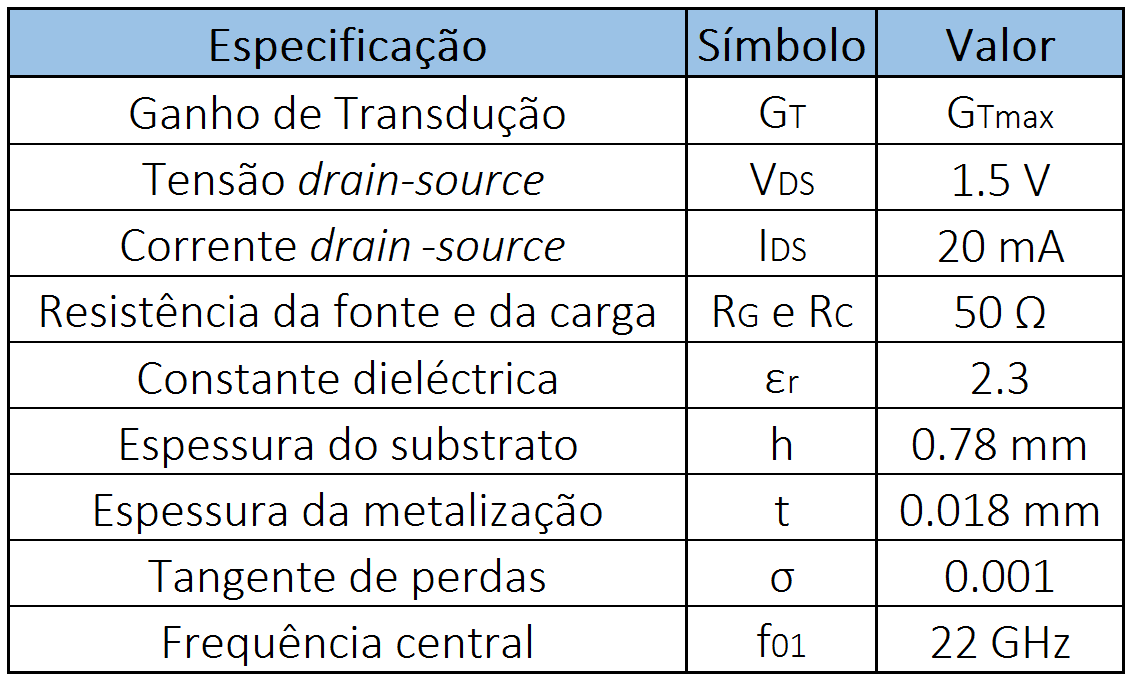
\includegraphics[keepaspectratio=true, scale=0.40]{teoricas/table1}
	\label{tab:car}
\end{table}

De notar que o valor da espessura do substrato foi modificado de 0.78 mm para 0.35 mm, com o objectivo de garantir propagação transversal nas linhas de microfita, ou seja, garantir que estas têm um comprimento maior que a largura. 

Numa primeira fase do trabalho laboratorial é projectado e simulado o amplificador uniandar com linhas simétricas. Na segunda fase o amplificador é projectado com tecnologia de microfita.

\subsection{Projecto de um amplificador uniandar}

\subsubsection{a) Projecto do amplificador com linhas ideais}

Nesta primeira fase, o amplificador é constituído pelo transístor descrito anteriormente, no entanto, todos os dispositivos utilizados no seu projecto e simulação são dispositivos ideais.

\paragraph{PFR Pretendido} \hspace{0pt} 

Em primeiro lugar, é feita uma análise DC ao transístor que tem em vista obter o ponto de funcionamento em repouso (PFR) especificado. O circuito que nos permitiu alcançar essa análise é o que se vê na Figura \ref{fig:Circuito_0}.

\begin{figure}[H]
	\centering
	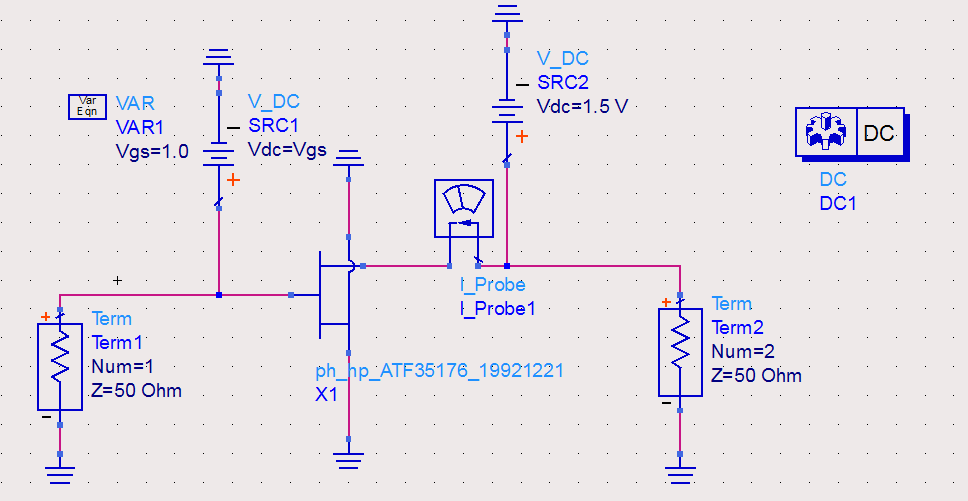
\includegraphics[keepaspectratio=true, scale=0.41]{exps/Circuito_0}
	\vspace{-0.5em}
	\caption{Circuito utilizado para obter o PFR desejado.}
	\label{fig:Circuito_0}
	\vspace{-0.8em}
\end{figure} 

A análise DC serve para descobrir o valor de $ V_{GS} $ correspondente ao PFR desejado. No circuito da Figura \ref{fig:Circuito_0} existe um componente denominado de \texttt{I\_Probe} que tem como objectivo controlar o valor de $ I_{D} $ à medida que o valor de $ V_{GS} $ varia. Um excerto dos resultados desta análise pode ser consultado na Figura \ref{fig:VGS}, onde se pode concluir que o valor da tensão  $V_{GS}$ que melhor corresponde a uma corrente $I_{D}$ de $20$ mA ($20.03$ mA) é de $-0.277$ V.

\begin{figure}[H]
	\centering
	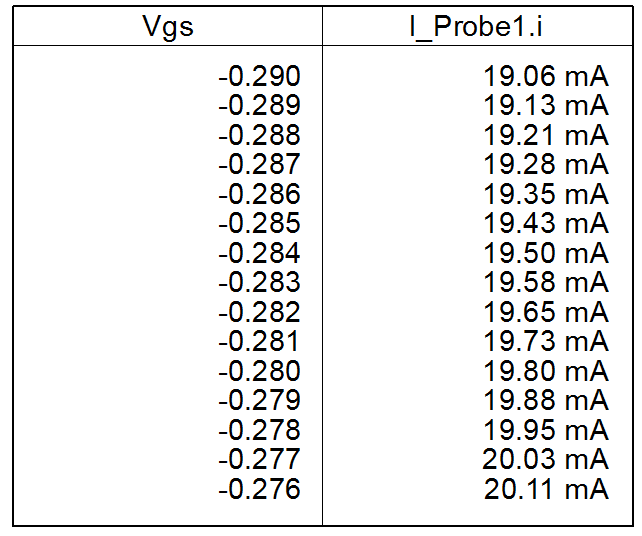
\includegraphics[keepaspectratio=true, scale=0.27]{exps/Vgs}
	\vspace{-0.5em}
	\caption{Valores de $V_{GS}$ correspondentes à corrente de \texttt{I\_Probe}.}
	\label{fig:VGS}
	\vspace{-0.8em}
\end{figure} 

\paragraph{Análise em Alta-Frequência} \hspace{0pt} 

Com o transístor a funcionar no PFR desejado, é preciso construir um novo circuito que contenha condensadores e bobines ideais, \texttt{DC\_Block} e \texttt{DC\_Feed}, respectivamente, para que seja possível realizar a simulação dos parâmetros S. Este circuito apresenta-se de seguida.

\begin{figure}[H]
	\centering
	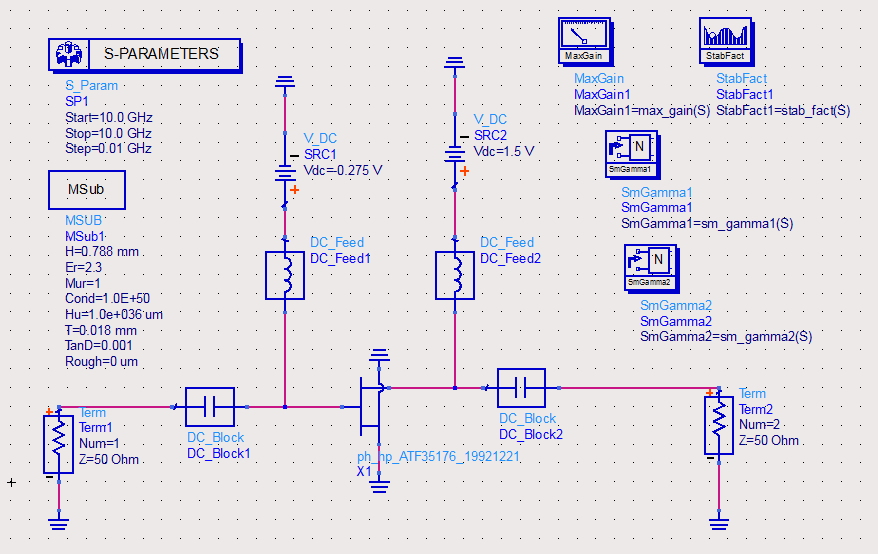
\includegraphics[keepaspectratio=true, scale=0.41]{exps/Circuito_1}
	\vspace{-0.5em}
	\caption{Circuito utilizado para obter o valores dos parâmetros S.}
	\label{fig:Circuito_1}
	\vspace{-0.8em}
\end{figure}

Simulando o circuito anteriormente projectado foram obtidos os seguintes valores para os parâmetros S, K (parâmetro de estabilidade), MAG (\textit{maximum available gain}) e para as cargas de adaptação para o transístor à frequência central.

\begin{table}[H]
 	\centering
 	\caption{Parâmetros que definem o transístor.}
 	\vspace{-1.5mm}
 	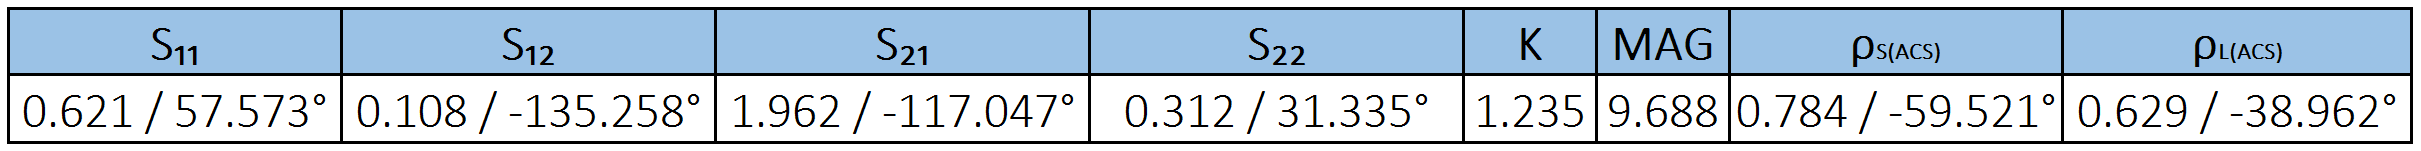
\includegraphics[keepaspectratio=true, scale=0.45]{teoricas/table2}
 	\label{tab:param_S}
\end{table}

De notar que os valores obtidos experimentalmente para os parâmetros S não podem ser verificados na \textit{datasheet} do transístor, uma vez que esta apenas especifica o comportamento do ATF-35176 para frequências entre 2 GHz e 18 GHz.

Com os valores da Tabela 2 determinados pode-se calcular o valor de $\Delta$, ou seja, o determinante da matriz de dispersão:

\vspace{-3mm}
\begin{equation}
\Delta = S_{11}S_{22} - S_{21}S_{12} = 0.067\angle-7.24 ^{\circ}.
\label{eq:delta}
\end{equation}

\vspace{1mm} 
Como se pode ver, K $= 1.236 > 1$, $\lvert \Delta \rvert = 0.067 < 1$ e $\lvert S_{ii} \rvert < 1$, pelo que o transístor é incondicionalmente estável.

\paragraph{Projecção da Malha de Entrada e de Saída} \hspace{0pt} 

Optou-se por projectar a malha de entrada e de saída com a Carta de Smith, recorrendo ao ADS. Como K $ > 1$ é possível efectuar adaptação conjugada simultânea (ACS) e, como se pretende adicionar elementos às malhas sabe-se que:

\vspace{-3mm}
\begin{equation}
\rho_{\text{in}} = \rho_{\text{S}}^{*} ~~ \text{e} ~~ \rho_{\text{out}} = \rho_{\text{L}}^{*}.
\end{equation}

\vspace{1mm} 
O circuito com malhas de adaptação é apresentado de seguida.

\begin{figure}[H]
	\centering
	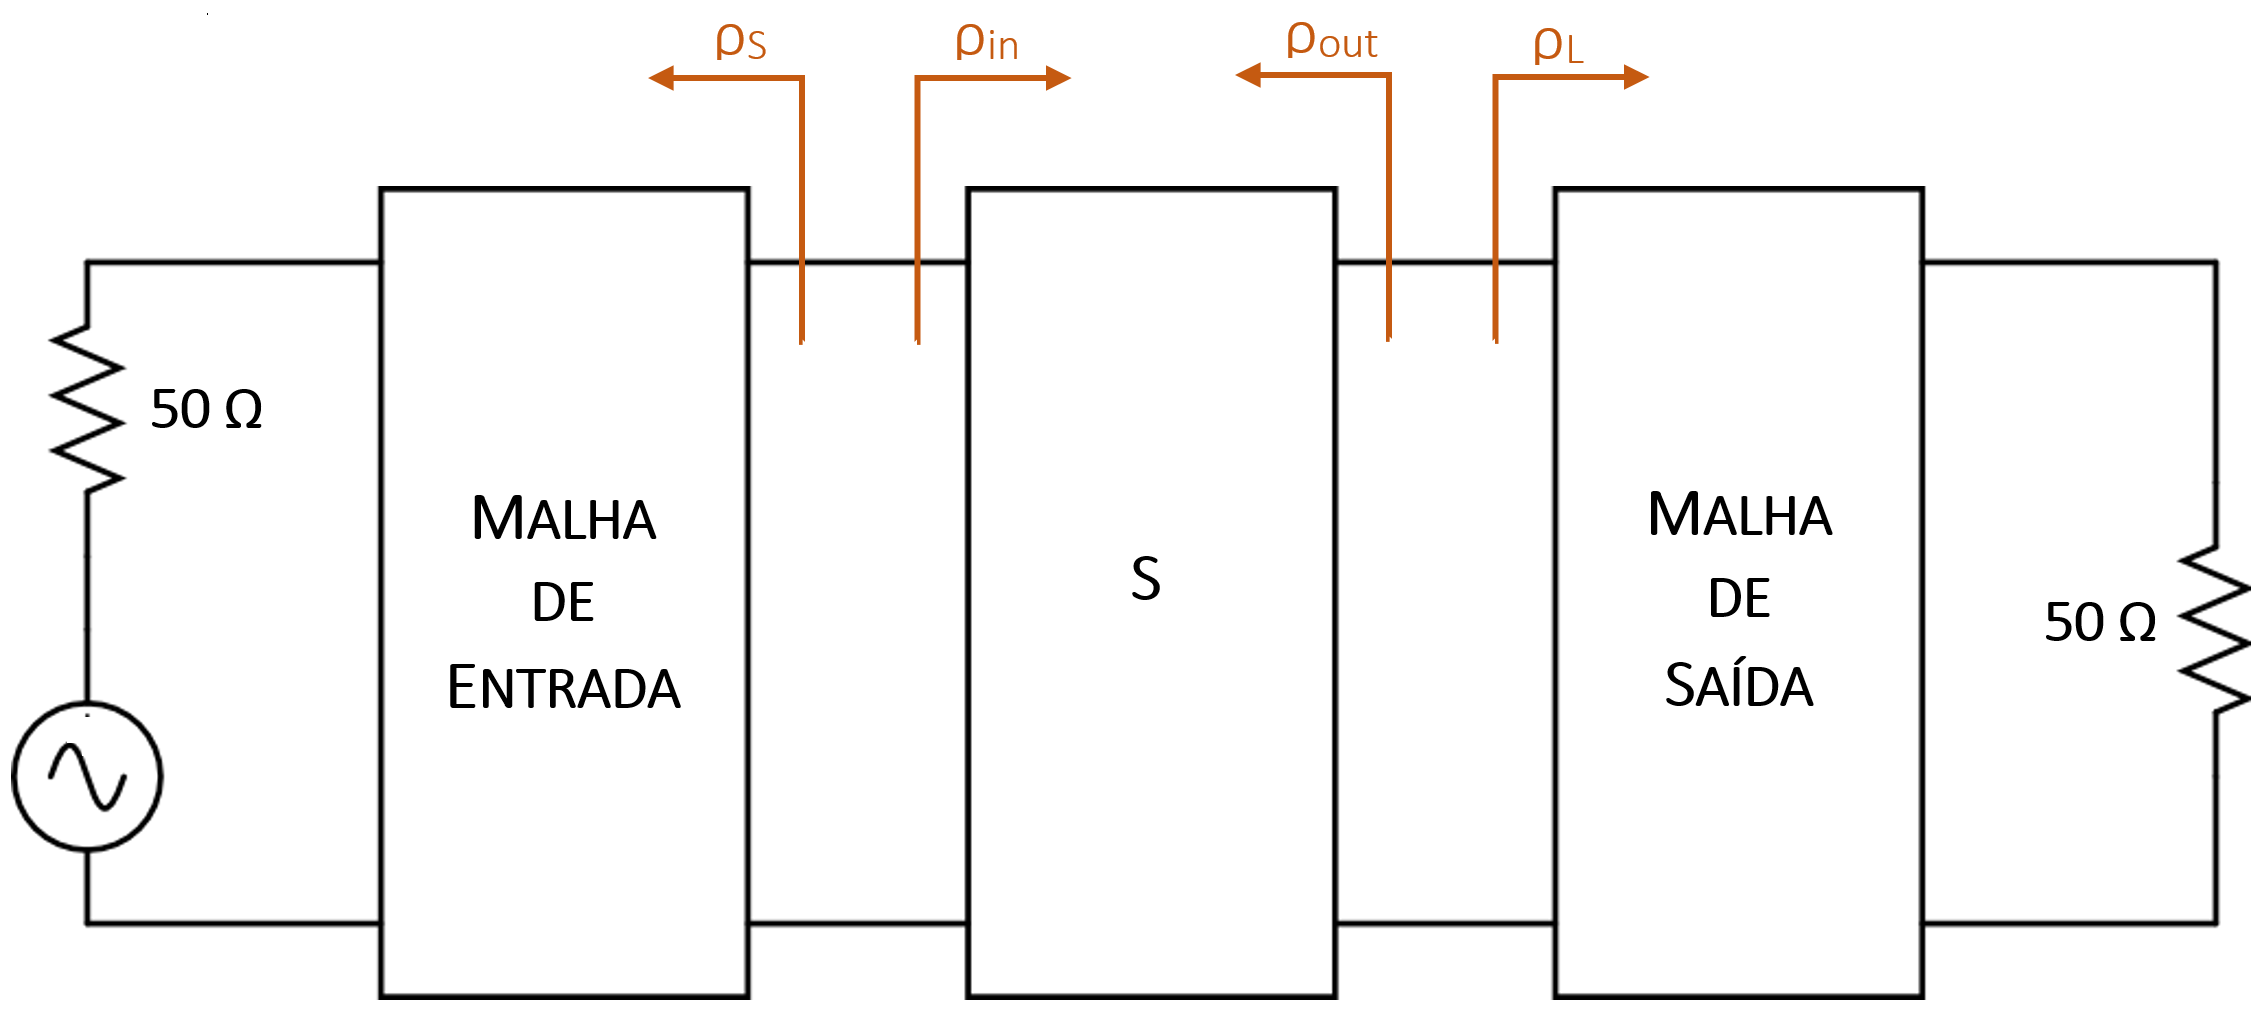
\includegraphics[keepaspectratio=true, scale=0.35]{teoricas/malhas}
	\vspace{-0.5em}
	\caption{Circuito que inclui as malhas de adaptação à entrada e à saída.}
	\vspace{-0.8em}
\end{figure}

Começando pela malha de entrada, ou seja, pelo gerador e sabendo que a malha de adaptação é do tipo linha-\textit{stub}, o circuito que se pretende projectar é da seguinte forma.

\begin{figure}[H]
	\centering
	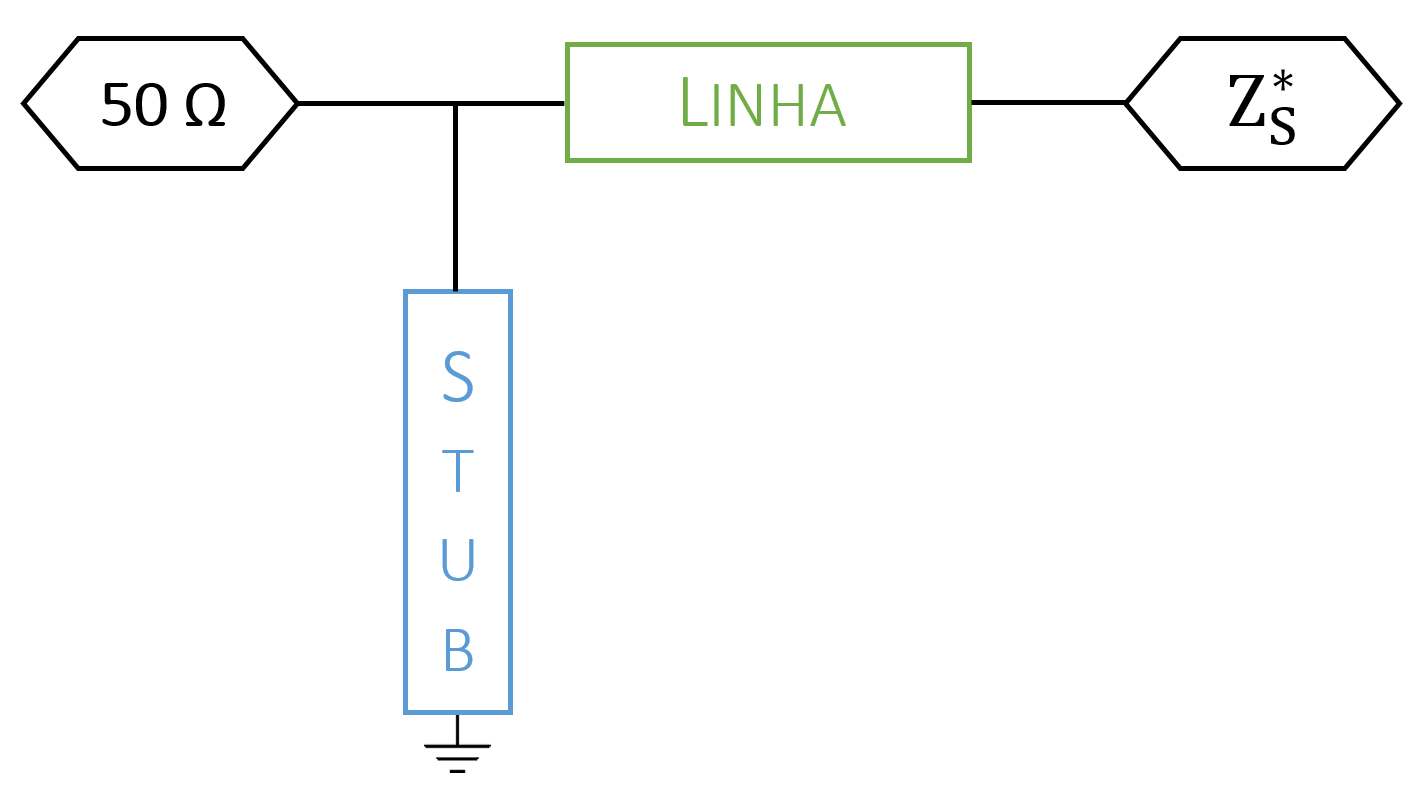
\includegraphics[keepaspectratio=true, scale=0.25]{teoricas/malhaentrada}
	\vspace{-0.5em}
	\caption{Malha de adaptação de entrada.}
	\vspace{-0.8em}
\end{figure}

Esta malha é construída com a adição de elementos, ou seja, \textit{towards generator}. O valor de $Z_{\text{S}}^{*}$ é de $0.784\angle59.529 ^{\circ}$.

No ADS, com recurso à Carta de Smith, determinou-se o comprimento eléctrico da linha de entrada, $\theta_{\text{L}_{\text{in}}}$, e o comprimento eléctrico do \textit{stub}, $\theta_{\text{S}_{\text{in}}}$. 

\begin{figure}[H]
	\centering
	\includegraphics[keepaspectratio=true, scale=0.45]{exps/Gerador_cc_line}
	\vspace{-0.5em}
	\caption{Determinação do comprimento eléctrico da linha de entrada - situação de CC.}
	\vspace{-0.8em}
\end{figure}

\begin{figure}[H]
	\centering
	\includegraphics[keepaspectratio=true, scale=0.45]{exps/Gerador_cc_stub}
	\vspace{-0.5em}
	\caption{Determinação do comprimento eléctrico do \textit{stub} de entrada - situação de CC.}
	\vspace{-0.8em}
\end{figure}

\vspace{-3mm}
\begin{equation}
	\theta_{\text{L}_{\text{in}}} = 100.494^{\circ}  ~~ \text{e} ~~ \theta_{\text{S}_{\text{in}}} = 21.751^{\circ}.
\end{equation}

\vspace{1mm} 
É de notar que os valores determinados anteriormente são para o \textit{stub} terminado em curto-circuito (CC), pois é nessa situação que o \textit{stub} é menor, tal como pretendido. Para verificar, optou-se por projectar a malha de entrada para o \textit{stub} terminado em circuito-aberto (CA).

\begin{figure}[H]
	\centering
	\includegraphics[keepaspectratio=true, scale=0.45]{exps/Gerador_Ca_line}
	\vspace{-0.5em}
	\caption{Determinação do comprimento eléctrico da linha de entrada - situação de CA.}
	\vspace{-0.8em}
\end{figure}

\begin{figure}[H]
	\centering
	\includegraphics[keepaspectratio=true, scale=0.45]{exps/Gerador_Ca_stub}
	\vspace{-0.5em}
	\caption{Determinação do comprimento eléctrico do \textit{stub} de entrada - situação de CA.}
	\vspace{-0.8em}
\end{figure}

Como se pode ver, para este caso o \textit{stub} é maior e, como tal, não é a solução preferível.

Olhando agora para a malha de saída, ou seja, para a carga e sabendo que a malha de adaptação é do tipo linha-\textit{stub}, o circuito que se pretende projectar é da seguinte forma.

\begin{figure}[H]
	\centering
	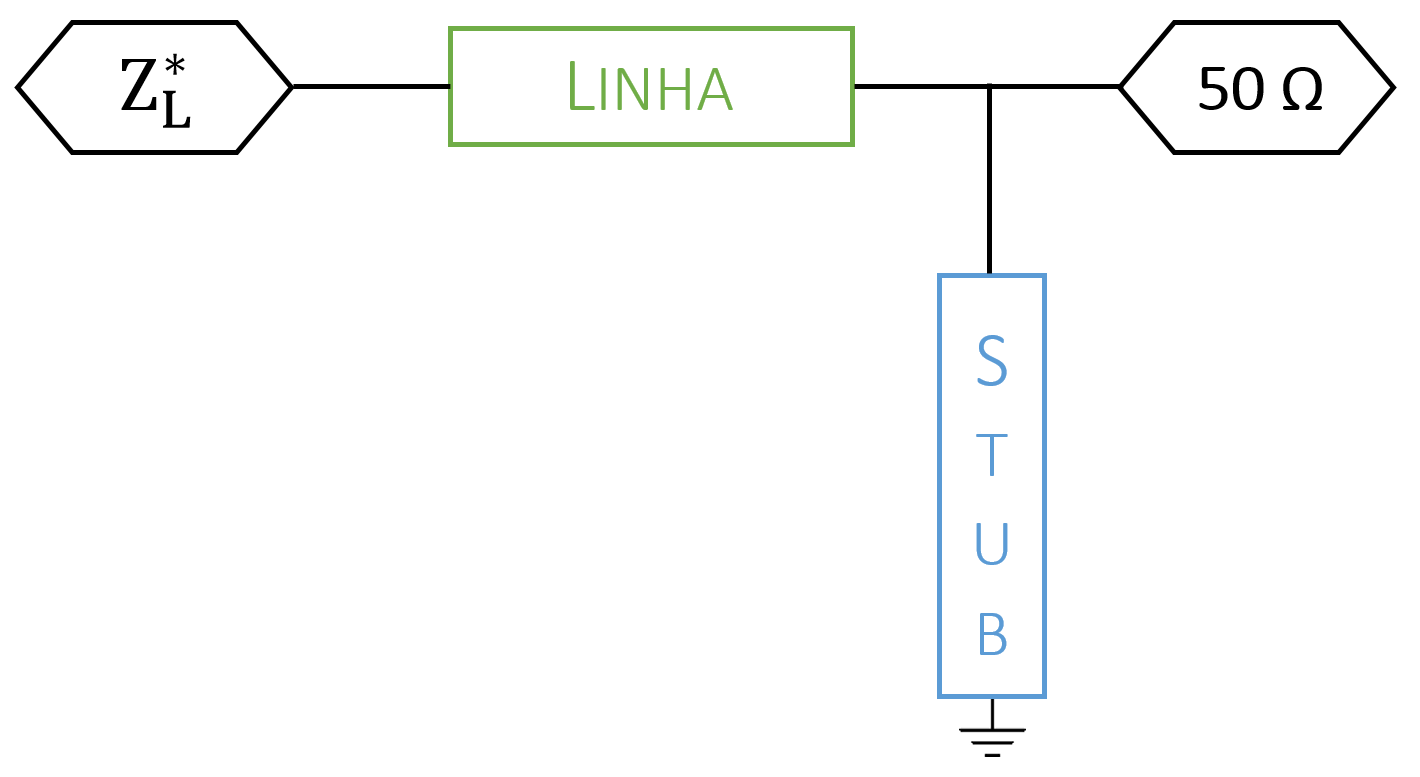
\includegraphics[keepaspectratio=true, scale=0.25]{teoricas/malhasaida}
	\vspace{-0.5em}
	\caption{Malha de adaptação de saída.}
	\vspace{-0.8em}
\end{figure}

Esta malha é construída com a adição de elementos, ou seja, \textit{towards generator}. O valor de $Z_{\text{L}}^{*}$ é de $0.628\angle39.020 ^{\circ}$.

No ADS, com recurso à Carta de Smith, determinou-se o comprimento eléctrico da linha, $\theta_{\text{L}_{\text{out}}}$, e o comprimento eléctrico do \textit{stub}, $\theta_{\text{S}_{\text{out}}}$. 

\begin{figure}[H]
	\centering
	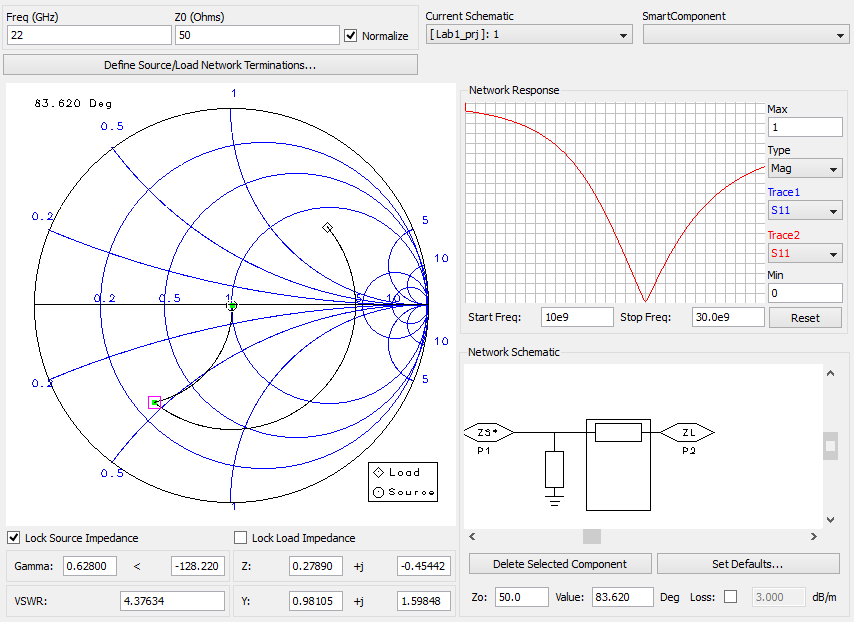
\includegraphics[keepaspectratio=true, scale=0.45]{exps/Carga_CC_line}
	\vspace{-0.5em}
	\caption{Determinação do comprimento eléctrico da linha de saída - situação de CC.}
	\vspace{-0.8em}
\end{figure}

\begin{figure}[H]
	\centering
	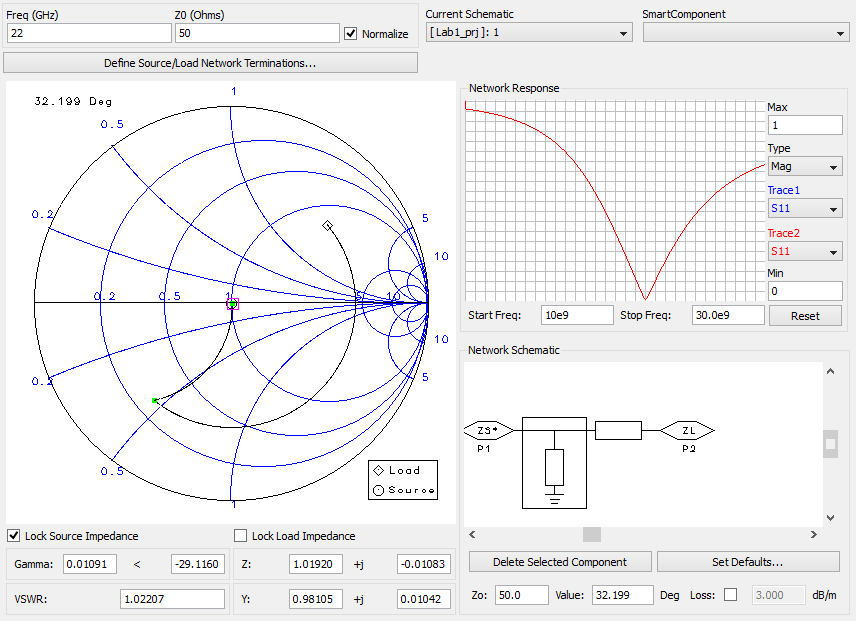
\includegraphics[keepaspectratio=true, scale=0.45]{exps/Carga_CC_stub}
	\vspace{-0.5em}
	\caption{Determinação do comprimento eléctrico do \textit{stub} de saída - situação de CC.}
	\vspace{-0.8em}
\end{figure}

\vspace{-3mm}
\begin{equation}
\theta_{\text{L}_{\text{out}}} = 83.620^{\circ}  ~~ \text{e} ~~ \theta_{\text{S}_{\text{out}}} = 32.199^{\circ}.
\end{equation}

\vspace{1mm} 

\paragraph{Simulação do Amplificador Ideal} \hspace{0pt}  

Após se obter através do ADS os valores dos comprimentos eléctricos dos dispositivos que compõem as malhas de adaptação de entrada e saída, pode-se então projectar um amplificador com malhas ideais, compostas por dispositivos sem perdas. O circuito projectado pode ser observado na Figura \ref{fig:circ_ideal}.

\begin{figure}[H]
	\centering
	\includegraphics[keepaspectratio=true, scale=0.41]{exps/Circuito_ideal}
	\vspace{-0.5em}
	\caption{Circuito do Amplificador com linhas ideais.}
	\vspace{-0.8em}
	\label{fig:circ_ideal}
\end{figure}
 
Após o circuito estar montado, as linhas ideais definidas com os seus comprimentos eléctricos e com frequência de referência centrada nos 22 GHz, foram realizadas várias simulações numa banda de frequências compreendida entre 10 GHz e 30 GHz de modo a obter os parâmetros pedidos, tal como se pode observar nas Figuras \ref{fig:ideal_estavel}, \ref{fig:ideal_S} e \ref{fig:ideal_noise}.

Em primeiro lugar testa-se a estabilidade do circuito a 22 GHz, estabilidade esta que, teoricamente, já tinha sido garantida com a Equação \ref{eq:delta} e com certos valores da Tabela \ref{tab:param_S}. Tal como se pode observar na Figura \ref{fig:ideal_estavel}, o parâmetro de estabilidade apresenta o valor esperado tabelado na Tabela \ref{tab:param_S}, confirmando a estabilidade do amplificador na frequência 22 GHz.

\begin{figure}[H]
	\centering
	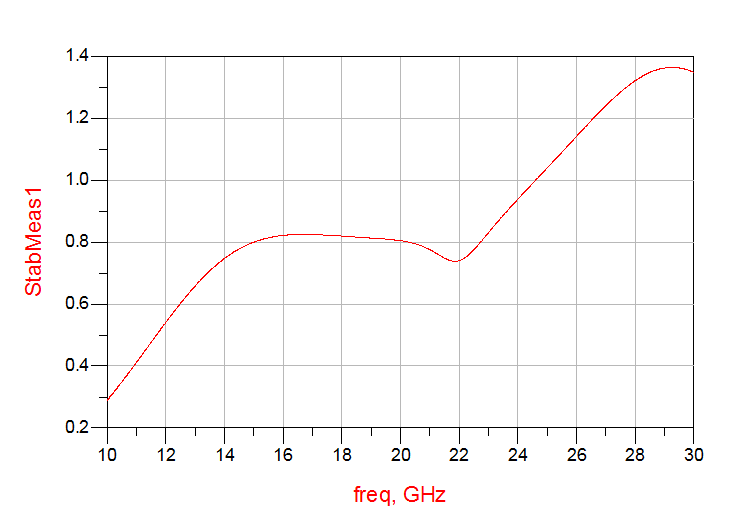
\includegraphics[keepaspectratio=true, scale=0.45]{exps/Ideal_estab}
	\vspace{-0.5em}
	\caption{Estabilidade do amplificador com linhas ideais.}
	\vspace{-0.8em}
	\label{fig:ideal_estavel}
\end{figure}

Através da simulação foi possível obter os parâmetros S, sendo que a parcela $S_{12}$ não representa uma característica relevante no amplificador e, por isso, não foi projectada. Ao observar a Figura \ref{fig:ideal_S}, e tendo em conta que a parcela $S_{11}$ representa o factor de reflexão à entrada, $S_{22}$ representa o factor de reflexão na saída e $S_{21}$ representa o ganho de transdução, podemos reparar que o amplificador está projectado para a frequência de 22 GHz, e que apresenta um valor para o ganho de transdução esperado.

\begin{figure}[H]
	\centering
	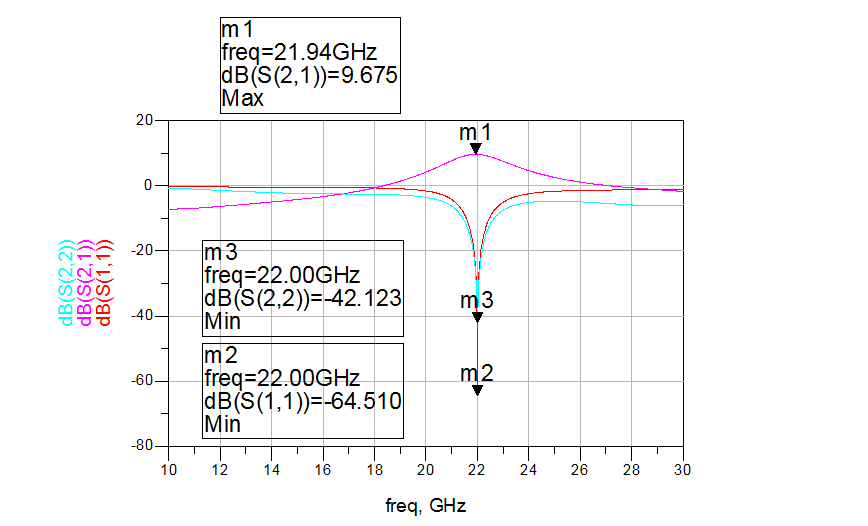
\includegraphics[keepaspectratio=true, scale=0.45]{exps/Ideal_S}
	\vspace{-0.5em}
	\caption{Parâmetros S do amplificador com linhas ideais.}
	\vspace{-0.8em}
	\label{fig:ideal_S}
\end{figure}

Foi também possível medir o \textit{noise} do amplificador ao longo da banda e, mais especificamente, na frequência de referência sobre a qual o amplificador irá operar, tal como se pode observar na Figura \ref{fig:ideal_noise}.

\begin{figure}[H]
	\centering
	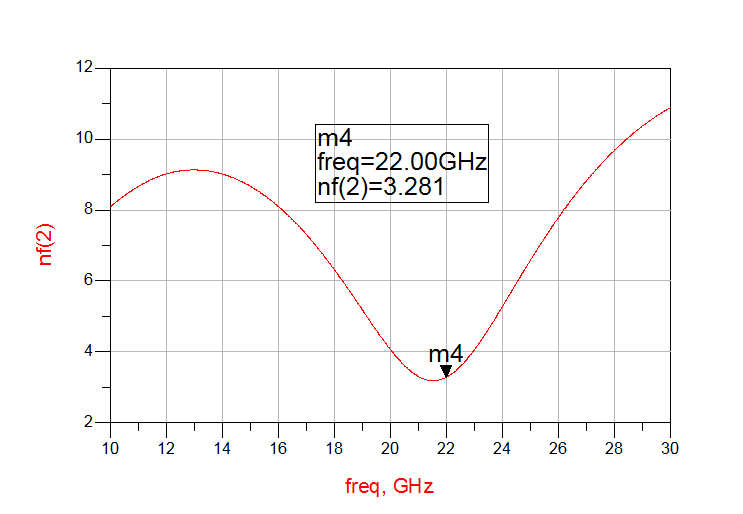
\includegraphics[keepaspectratio=true, scale=0.45]{exps/Ideal_noise}
	\vspace{-0.5em}
	\caption{Factor de ruído no amplificador com linhas ideais.}
	\vspace{-0.8em}
	\label{fig:ideal_noise}
\end{figure}

Das simulações anteriores foram obtidos os seguintes resultados.

\begin{table}[H]
	\centering
	\caption{Parâmetros experimentais que definem o transístor quando projectado com linhas ideais.}
	\vspace{-1.5mm}
	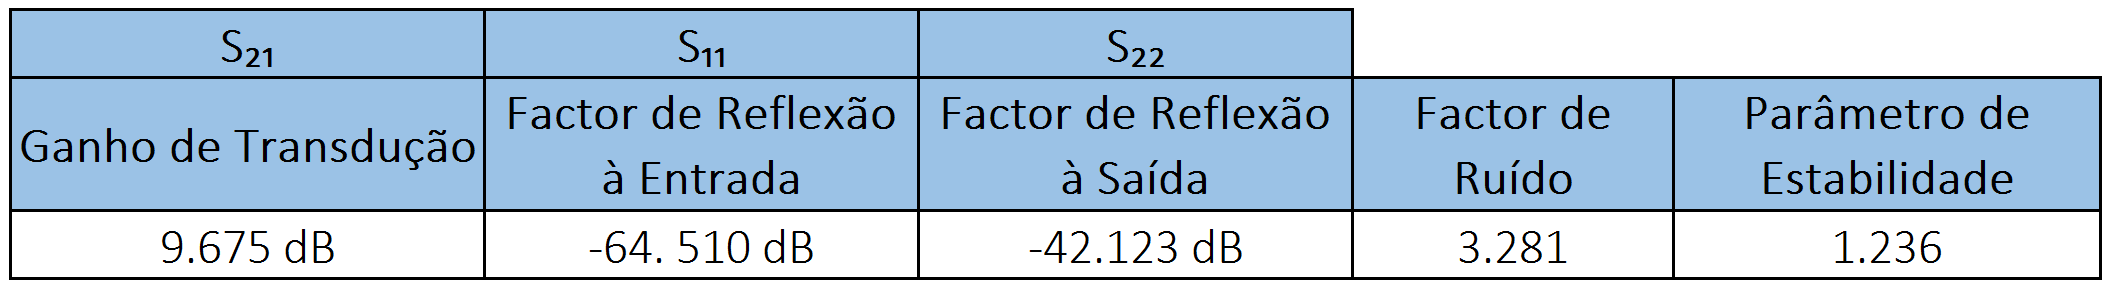
\includegraphics[keepaspectratio=true, scale=0.45]{exps/pergunta4}
\end{table}

\todo{Tirar conclusões sobre isto, mas poucas isto é tipo a experiência base, o ideal, se calhar explicava-se o que significa cada coisa. é para comparar com a teoria?}

\subsubsection{b) Projecto do amplificador utilizando tecnologia microfita}

Tendo já completado o projecto do amplificador com linha ideais, tem-se agora as características ideais que representam um objectivo que se tenta alcançar. É de referir que no caso ideal não foram considerados quaisquer tipo de perdas e, assim, o amplificador real será diferente.

Em primeiro lugar os blocos \texttt{DC\_Block} e \texttt{DC\_Feed} terão de ser substituídos por dispositivos reais com valores reais, condensadores e bobines respectivamente. 

No caso do condensador de desacoplamento, $C_{D}$, o seu valor tem de cumprir a condição especificada na equação \ref{eq:cond_cap}, pois sabe-se que a impedância dos condensadores de desacoplamento deve ser bastante inferior à impedância característica das linhas de transmissão. 

\vspace{-3mm}
\begin{equation}
\lvert Z_C \rvert = \frac{1}{w_{0} C_{D}} << Z_0 \hspace{2mm} \rightarrow \hspace{2mm} C_{D} > \frac{1}{w_{0}Z_0 \times 0.1} \hspace{2mm} \rightarrow \hspace{2mm} C_{D} > \dfrac{1}{5 \times 2 \pi \times 22 \times 10^{9}} = 1.45~\text{pF}.
\label{eq:cond_cap}
\end{equation}

\vspace{1mm}
No caso da bobine de bloqueio, $L_{CHK}$, o seu valor tem de cumprir a condição especificada na Equação \ref{eq:cond_ind}, pois sabe-se que a impedância das bobines de bloqueio deve ser bastante superior à impedância característica das linhas de transmissão.  

\vspace{-3mm}
\begin{equation}
\lvert Z_L \rvert = w_{0} L_{CHK} >> Z_0 \hspace{2mm} \rightarrow \hspace{2mm} L_{CHK} > \frac{Z_0 \times 10}{w_{0}} \hspace{2mm} \rightarrow \hspace{2mm} L_{CHK} > \frac{500}{2 \pi \times 22 \times 10^{9}} = 3.62~\text{nH}.
\label{eq:cond_ind}
\end{equation}

\vspace{1mm}
Tendo escolhido valores que correspondam a condensadores e bobines que existam no mercado, o valor de $L_{CHK}$ é de 3.9 nH e o valor de $C_{D}$ é de 10 pF. No entanto, com o avanço do laboratório o valor de $C_{D}$ foi alterado para 39 pF pois com este valor as simulações apresentavam melhores resultados.

Em segundo lugar, é necessário de substituir as linhas ideais por dispositivos reais, dispositivos estes que representam a tecnologia microfita utilizada no amplificador. Para tal, recorre-se à ferramenta \texttt{LineCalc} do ADS, como se pode ver na Figura \ref{fig:LineCalc}, para calcular as dimensões das microfitas a utilizar. É necessário colocar as características do substrato, Tabela \ref{tab:car}, a frequência de referência e finalmente a impedância e comprimento eléctrico desejados para a microfita.

\begin{figure}[H]
	\centering
	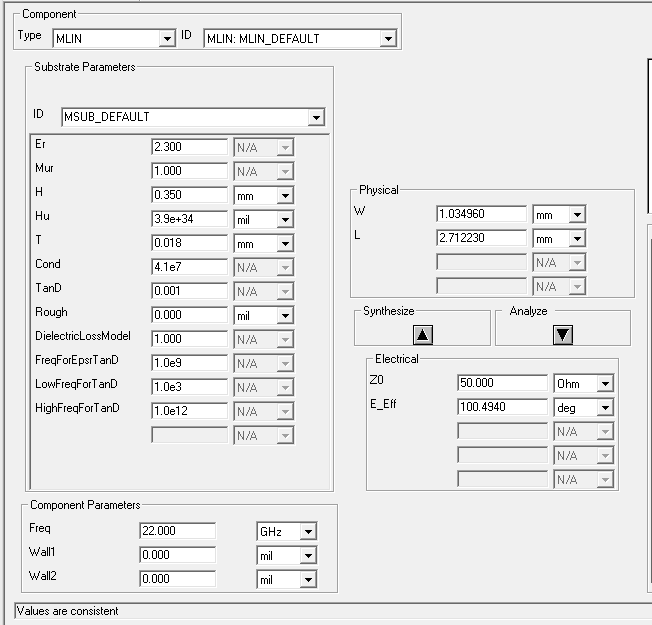
\includegraphics[keepaspectratio=true, scale=0.35]{exps/LineCalc}
	\vspace{-0.5em}
	\caption{\texttt{LineCalc} feito para a linha da malha de adaptação de entrada.}
	\vspace{-0.8em}
	\label{fig:LineCalc}
\end{figure}

Numa primeira fase, as malhas de adaptação foram construídas com os elementos \texttt{MLIN} (linhas) e \texttt{MLSC} (\textit{stubs}) estando o circuito representado na Figura \ref{fig:mf_stub_circuito} e os seus parâmetros S na Figura \ref{fig:mf_stub_S}.

\begin{figure}[H]
	\centering
	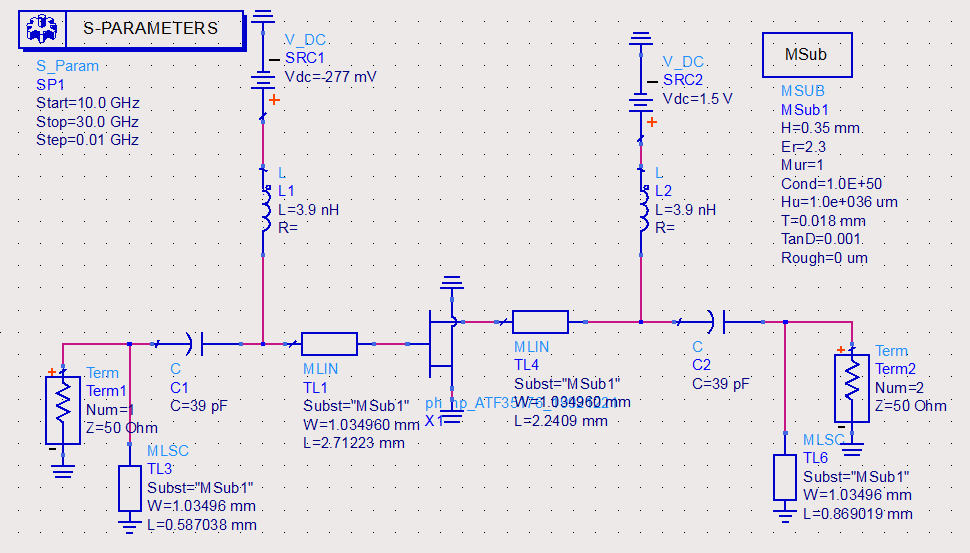
\includegraphics[keepaspectratio=true, scale=0.45]{exps/Circuito_mf_stub}
	\vspace{-0.5em}
	\caption{Circuito com microfitas, linhas e \textit{stubs}.}
	\vspace{-0.8em}
	\label{fig:mf_stub_circuito}
\end{figure}

\begin{figure}[H]
	\centering
	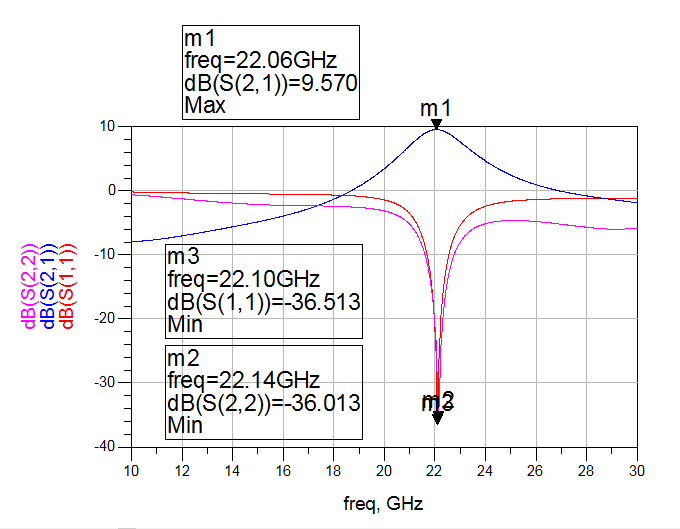
\includegraphics[keepaspectratio=true, scale=0.45]{exps/mf_stub_S}
	\vspace{-0.5em}
	\caption{Parâmetros S do amplificador com malhas linha-\textit{stub}.}
	\vspace{-0.8em}
	\label{fig:mf_stub_S}
\end{figure}

Os resultados desta simulação são bastante satisfatórios, no entanto, como foi explicado anteriormente na Secção \ref{sec:Pla_Trab}, não será possível utilizar este circuito. Ao observarmos as dimensões dos dispositivos \texttt{MLSC}, reparamos que a sua largura é superior ao seu comprimento, tendo então de representar estes elementos com outros dispositivos, \texttt{MLOC}. Ao dimensionar \texttt{MLOC}, no entanto, o comprimento eléctrico considerado tem de ser incrementado em $90^{\circ}$. Um exemplo da progressão do processo da dimensão do \textit{stub} da malha de adaptação pode ser observado na Figura \ref{fig:stub_fail}.

\begin{figure}[H]
	\centering
	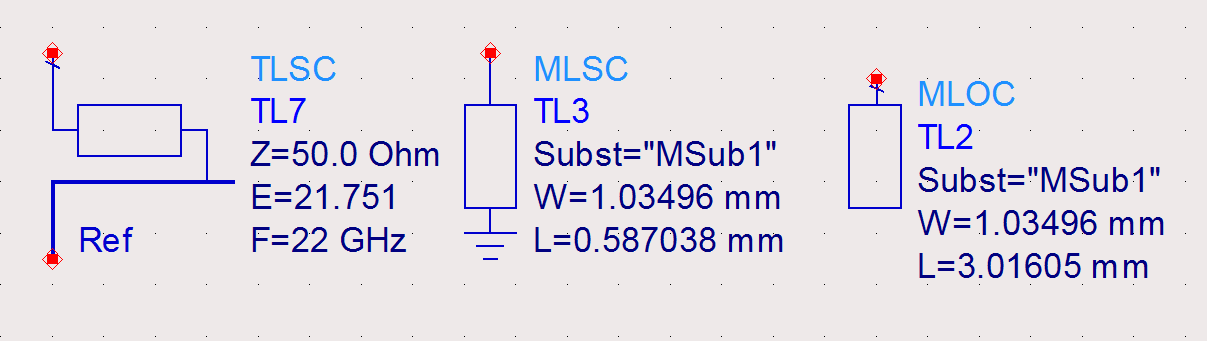
\includegraphics[keepaspectratio=true, scale=0.3]{exps/stub_fail}
	\vspace{-0.5em}
	\caption{Representado na direita está a linha ideal (\texttt{TLSC}), no meio o \textit{stub} (\texttt{MLSC}) e na esquerda o \textit{loc} (\texttt{MLOC}).}
	\vspace{-0.8em}
	\label{fig:stub_fail}
\end{figure}

Com esta modificação obtém-se um circuito diferente do anterior, Figura \ref{fig:circuito_mf}, onde se testa os seus parâmetros, tal como feito para o circuito com linhas ideais, Figura \ref{fig:circ_ideal}. Estas simulações estão representadas nas Figuras \ref{fig:mf_est}, \ref{fig:mf_S} e \ref{fig:mf_noise}.

\begin{figure}[H]
	\centering
	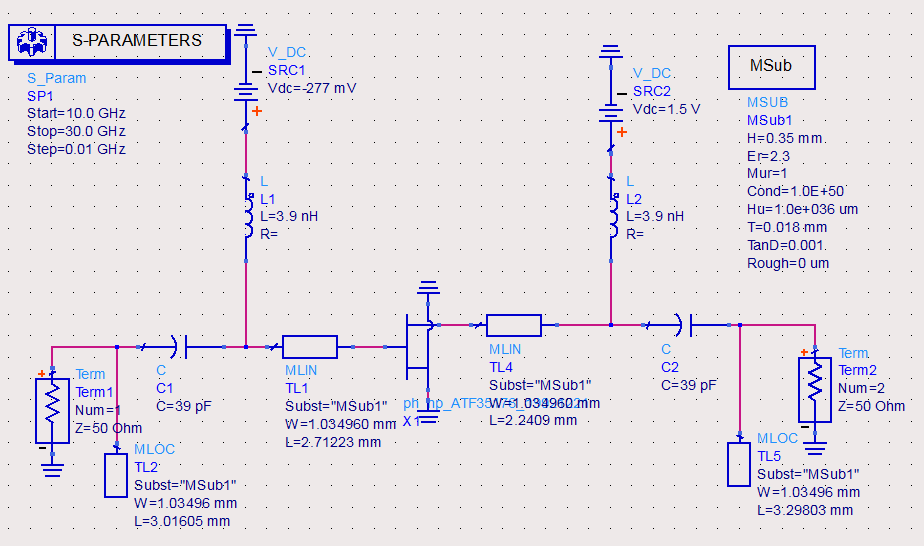
\includegraphics[keepaspectratio=true, scale=0.41]{exps/Circuito_mf}
	\vspace{-0.5em}
	\caption{Circuito com microfitas, linhas e \textit{locs}.}
	\vspace{-0.8em}
	\label{fig:circuito_mf}
\end{figure}

Como se pode observar na Figura \ref{fig:mf_est} (a escala da figura foi ajustada de modo a permitir uma melhor observação da evolução do parâmetro de estabilidade), e em comparação com o que se verifica na Figura \ref{fig:ideal_estavel}, o parâmetro de estabilidade para 22 GHz apresenta um erro relativo baixo e garante a estabilidade do amplificador para 22GHz.

\todo{Verificar estabilidade em banda larga.}

\begin{figure}[H]
	\centering
	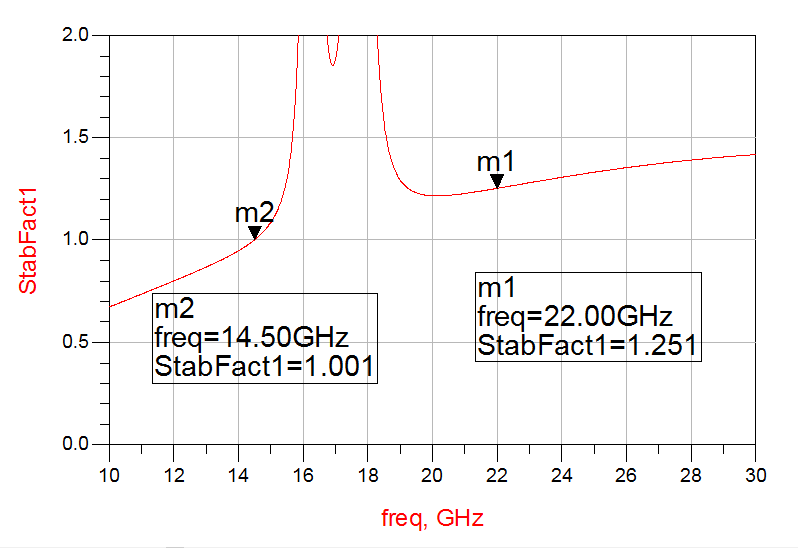
\includegraphics[keepaspectratio=true, scale=0.41]{exps/mf_estab}
	\vspace{-0.5em}
	\caption{Estabilidade do amplificador com malhas de linhas e \textit{locs}.}
	\vspace{-0.8em}
	\label{fig:mf_est}
\end{figure}

Na Figura \ref{fig:mf_S} verifica-se que os gráficos apresentam uma forma muito diferente da apresentada antes da alteração nos \textit{stubs}, Figura \ref{fig:mf_stub_S}, sendo esta mudança também verificada na Figura \ref{fig:mf_noise}. Ambos os gráficos não apresentam a forma esperada aquando da simulação do amplificador com linhas ideais, efeito causado pela alteração realizada nos \textit{stubs}.

\begin{figure}[H]
	\centering
	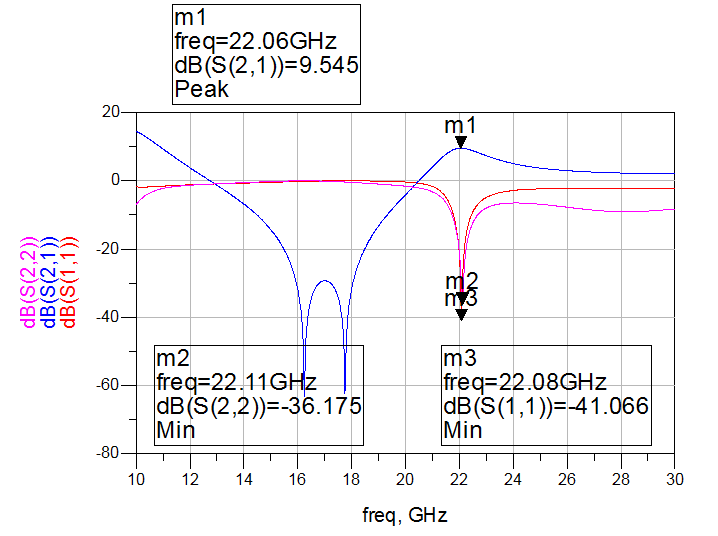
\includegraphics[keepaspectratio=true, scale=0.45]{exps/mf_S}
	\vspace{-0.5em}
	\caption{Parâmetros S do amplificador com malhas de linhas e \textit{locs}.}
	\vspace{-0.8em}
	\label{fig:mf_S}
\end{figure}

\begin{figure}[H]
	\centering
	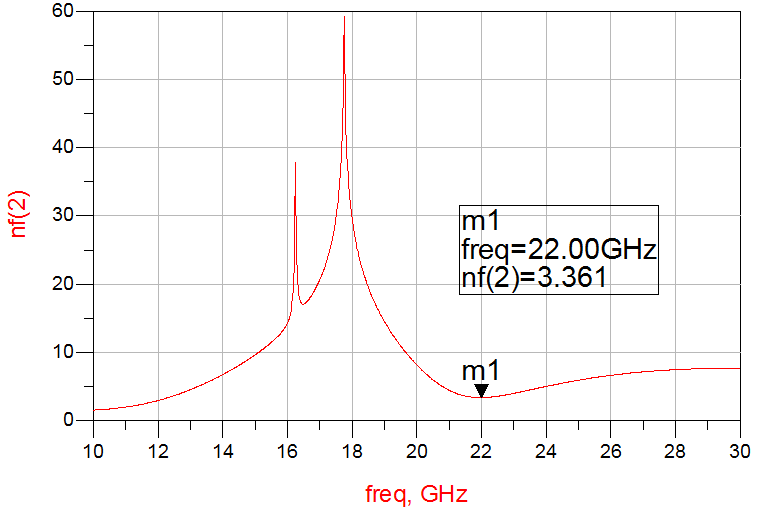
\includegraphics[keepaspectratio=true, scale=0.45]{exps/mf_noise}
	\vspace{-0.5em}
	\caption{Factor de ruído no amplificador com malhas de linhas e \textit{locs}.}
	\vspace{-0.8em}
	\label{fig:mf_noise}
\end{figure}

Na tabela abaixo encontra-se uma tabela com uma síntese dos parâmetros do amplificador quando projectado com linhas ideais e com microfita.

\begin{table}[H]
	\centering
	\caption{Parâmetros experimentais que definem o amplificador quando projectado com linhas ideais e tecnologia microfita.}
	\vspace{-1.5mm}
	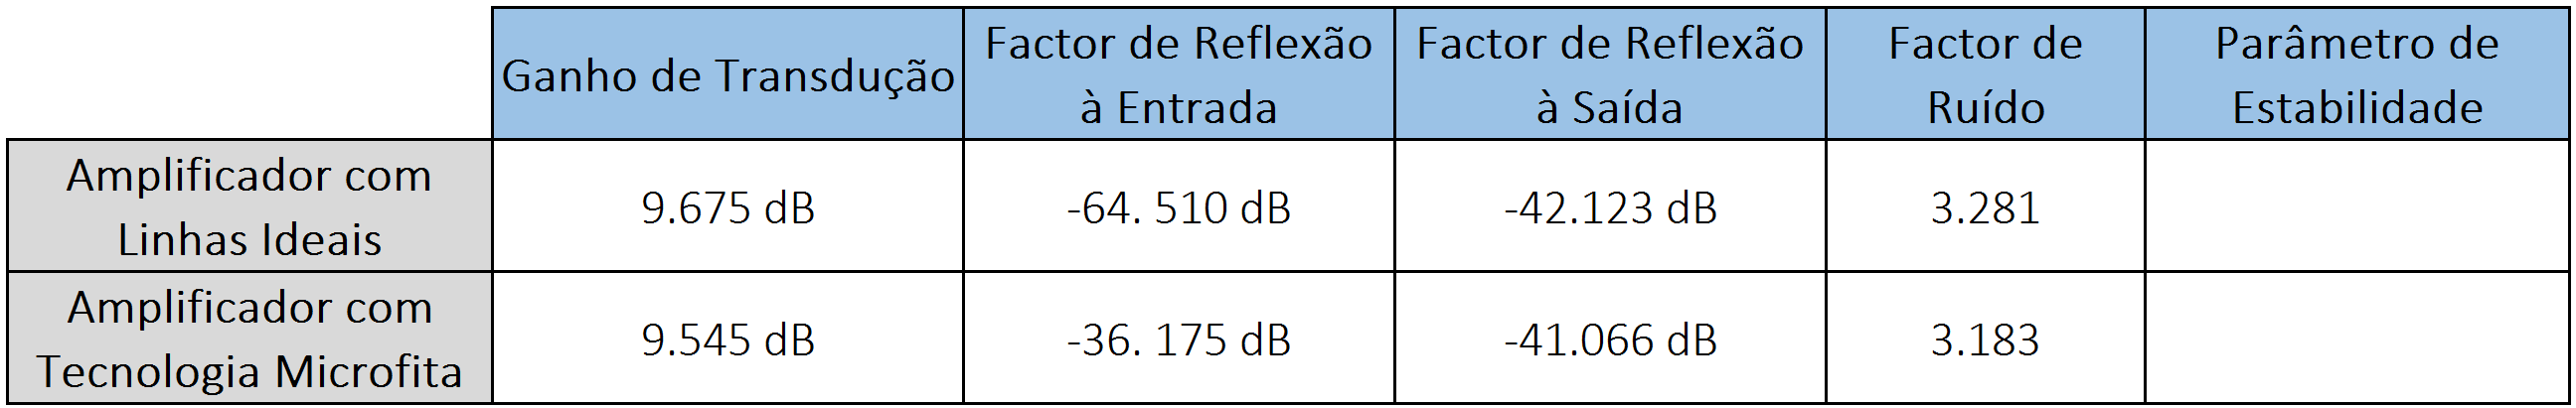
\includegraphics[keepaspectratio=true, scale=0.45]{exps/comparacaoamp}
	\label{tab:comparacao}
\end{table}

A diferença entre os gráficos obtidos no amplificador de linhas ideais (Figuras \ref{fig:ideal_estavel}, \ref{fig:ideal_S} e \ref{fig:ideal_noise}) e o amplificador com a tecnologia de microfita (Figuras \ref{fig:mf_est}, \ref{fig:mf_S} e \ref{fig:mf_noise}) são relevantes, especialmente em zonas perto das frequências 16 GHz e 18 GHz. No entanto, a maior parte dos valores que se obtêm para a frequência de 22 GHz não apresentam diferenças tão relevantes, tal como se pode observar na Tabela \ref{tab:comparacao}. O valor do factor de reflexão à entrada tem uma queda no valor do módulo para quase metade, no entanto, essa diferença não terá um efeito tão significativo no funcionamento do amplificador. No amplificador com linhas ideais, o factor de reflexão com menor módulo é o factor de reflexão à saída, com um valor de $-42.123$ dB, no entanto, no amplificador com tecnologia de microfita, já é o factor de reflexão à entrada que apresenta o menor módulo, tomando o valor de $-36.175$ dB. É esta alteração de valores que é relevante para o funcionamento do circuito, e que pode ser justificada, tal como as outras diferenças entre os amplificadores, com as perdas nas microfitas.

\subsection{Concretização do amplificador em tecnologia de microfita}

Nesta segunda fase o circuito do amplificador será todo projectado com a tecnologia de microfita e irá ser projectado um \textit{layout} do circuito.

\subsubsection{a) Introdução de elementos que simulam descontinuidades nas linhas}

Em primeiro lugar, substitui-se ambas as bobines e as suas fontes de tensão pelo bloco demonstrado na Figura \ref{fig:bobine}, isto de modo a utilizar tecnologia de microfita para simular as bobines. 

\begin{figure}[H]
	\centering
	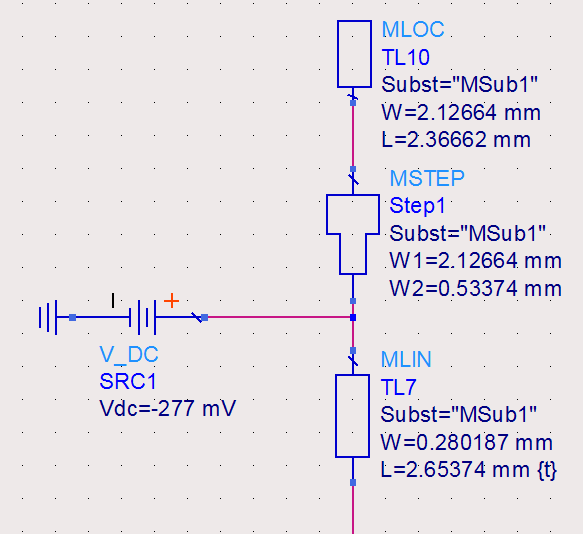
\includegraphics[keepaspectratio=true, scale=0.45]{exps/bobine}
	\vspace{-0.5em}
	\caption{Bloco que substitui bobines e fontes de tensão.}
	\vspace{-0.8em}
	\label{fig:bobine}
\end{figure}

O elemento \texttt{MLIN} com o nome de \texttt{TL7} representado na Figura \ref{fig:bobine} tem dimensões obtidas através da ferramenta \texttt{LineCalc} já antes utilizada, no entanto, como argumentos, recebe impedância característica de $100 \Omega$ e comprimento eléctrico de $90^{\circ}$. O elemento \texttt{MLIN} com o nome de \texttt{TL8} tem dimensões calculadas através do mesmo método, no entanto, recebe como impedância característica um valor de $30 \Omega$. Esta alteração no cálculo das dimensões dos elementos \texttt{MLIN} irá causar uma diferença na largura de ambos, sendo necessário usar um elemento \texttt{MSTEP} que tem como objectivo servir de ``adaptador'' para a diferença das larguras entre os canais.

Em relação às quatro descontinuidades criadas nos nós dos circuitos serão usados elementos \texttt{MTEE} que terão como função criar uma junção entre três canais e também, se necessário, adaptar as suas larguras. O resultado destas modificações no circuito do amplificador podem ser observadas na Figura \ref{fig:Circuito_pre_tune}.

\begin{figure}[H]
	\centering
	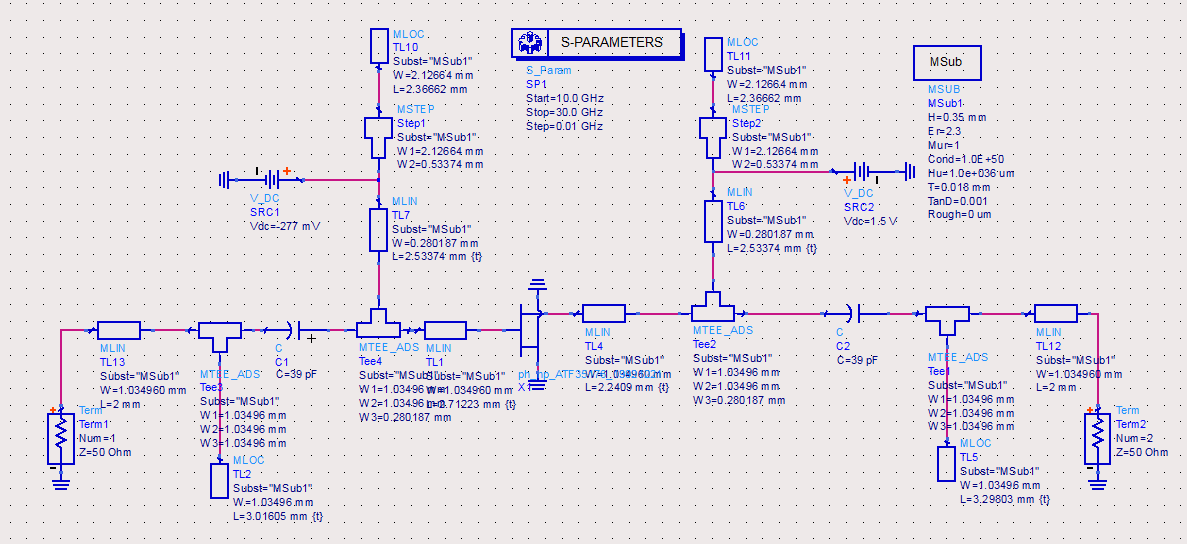
\includegraphics[keepaspectratio=true, scale=0.45]{exps/Circuito_descont_pre_tune}
	\vspace{-0.5em}
	\caption{Amplificador com as descontinuidades simuladas.}
	\vspace{-0.8em}
	\label{fig:Circuito_pre_tune}
\end{figure}

Após ter o circuito projectado é possível observar os parâmetros S, Figura \ref{fig:descont_S_pre_tune}, que caracterizam o amplificador.

\begin{figure}[H]
	\centering
	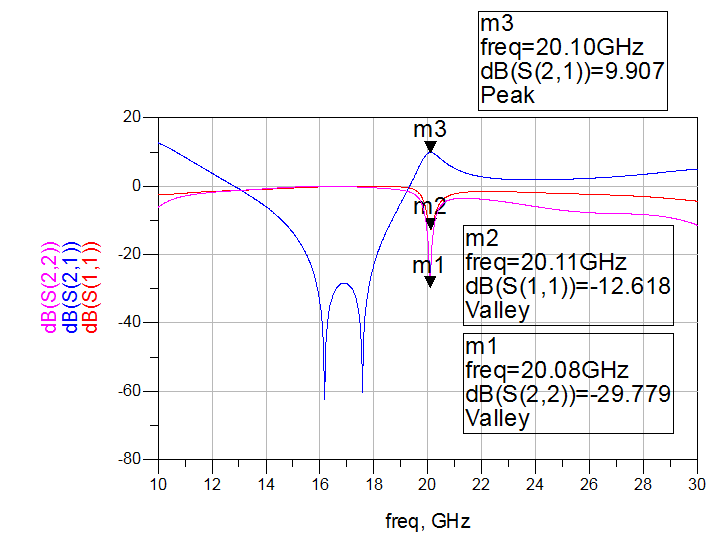
\includegraphics[keepaspectratio=true, scale=0.45]{exps/descont_S_pre_tune}
	\vspace{-0.5em}
	\caption{Simulação dos parâmetros S do amplificador com descontinuidades simuladas pré-\texttt{TUNE}.}
	\vspace{-0.8em}
	\label{fig:descont_S_pre_tune}
\end{figure}

Como se pode observar, os resultados obtidos não são satisfatórios, os valores máximos/mínimos não se encontram centrados na frequência desejada e não apresentam valores tão próximos do esperado. Assim, foi utilizada a ferramenta \texttt{TUNE} nos comprimentos dos elementos \texttt{MLIN} com o nome de \texttt{TL2}, \texttt{TL1}, \texttt{TL4}, \texttt{TL5}, \texttt{TL7}, \texttt{TL10}, \texttt{TL6} e \texttt{TL11} representados na Figura \ref{fig:Circuito_pre_tune}, onde foi possível obter as características representadas na Figura \ref{fig:descont_S_pos_tune}.

\begin{figure}[H]
	\centering
	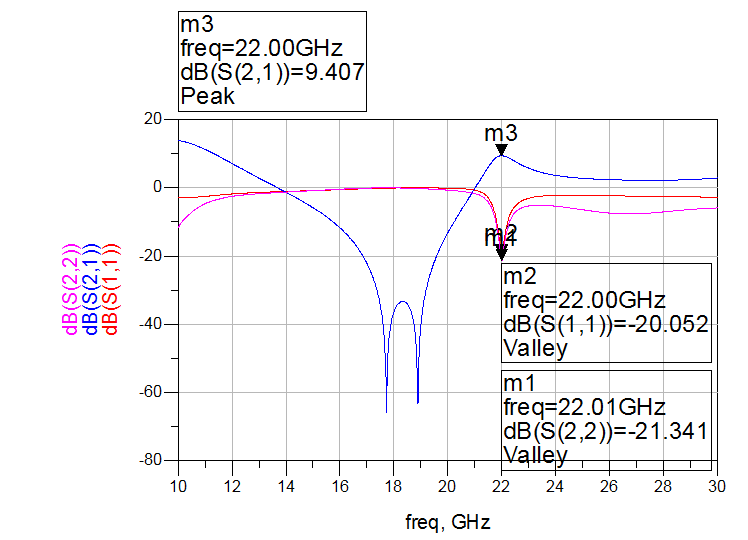
\includegraphics[keepaspectratio=true, scale=0.45]{exps/descont_S_pos_tune}
	\vspace{-0.5em}
	\caption{Simulação dos parâmetros S do amplificador com descontinuidades simuladas pós-\texttt{TUNE}.}
	\vspace{-0.8em}
	\label{fig:descont_S_pos_tune}
\end{figure}

\begin{figure}[H]
	\centering
	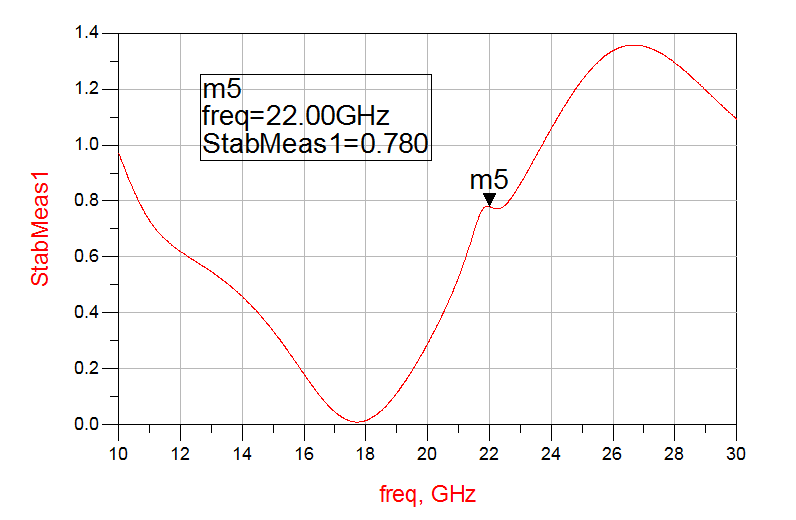
\includegraphics[keepaspectratio=true, scale=0.45]{exps/descont_estab_pos_tune}
	\vspace{-0.5em}
	\caption{Estabilidade do amplificador com descontinuidades simuladas pós-\texttt{TUNE}.}
	\vspace{-0.8em}
	\label{fig:descont_estab_pos_tune}
\end{figure}

\begin{figure}[H]
	\centering
	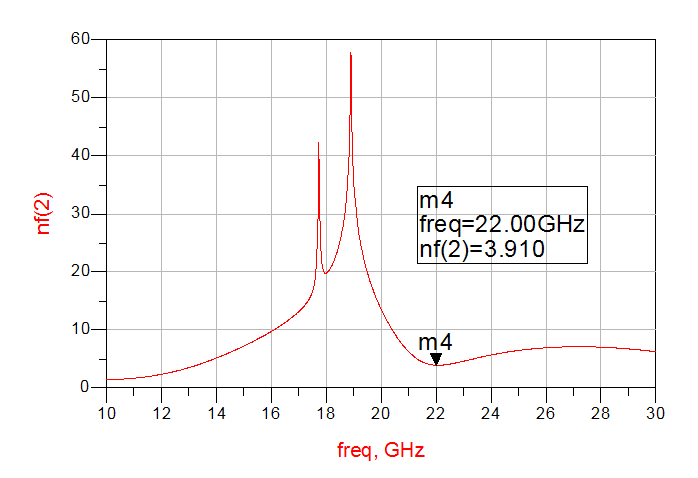
\includegraphics[keepaspectratio=true, scale=0.45]{exps/descont_noise_pos_tune}
	\vspace{-0.5em}
	\caption{Factor de ruído no amplificador com descontinuidades simuladas pós-\texttt{TUNE}.}
	\vspace{-0.8em}
	\label{fig:descont_noise_pos_tune}
\end{figure}

Na Tabela \ref{tab:comparacao_final} está uma comparação entre os vários métodos utilizados para projectar o amplificador.

\begin{table}[H]
	\centering
	\caption{Comparação dos parâmetros que definem o amplificador entre vários métodos de implementação.}
	\vspace{-1.5mm}
	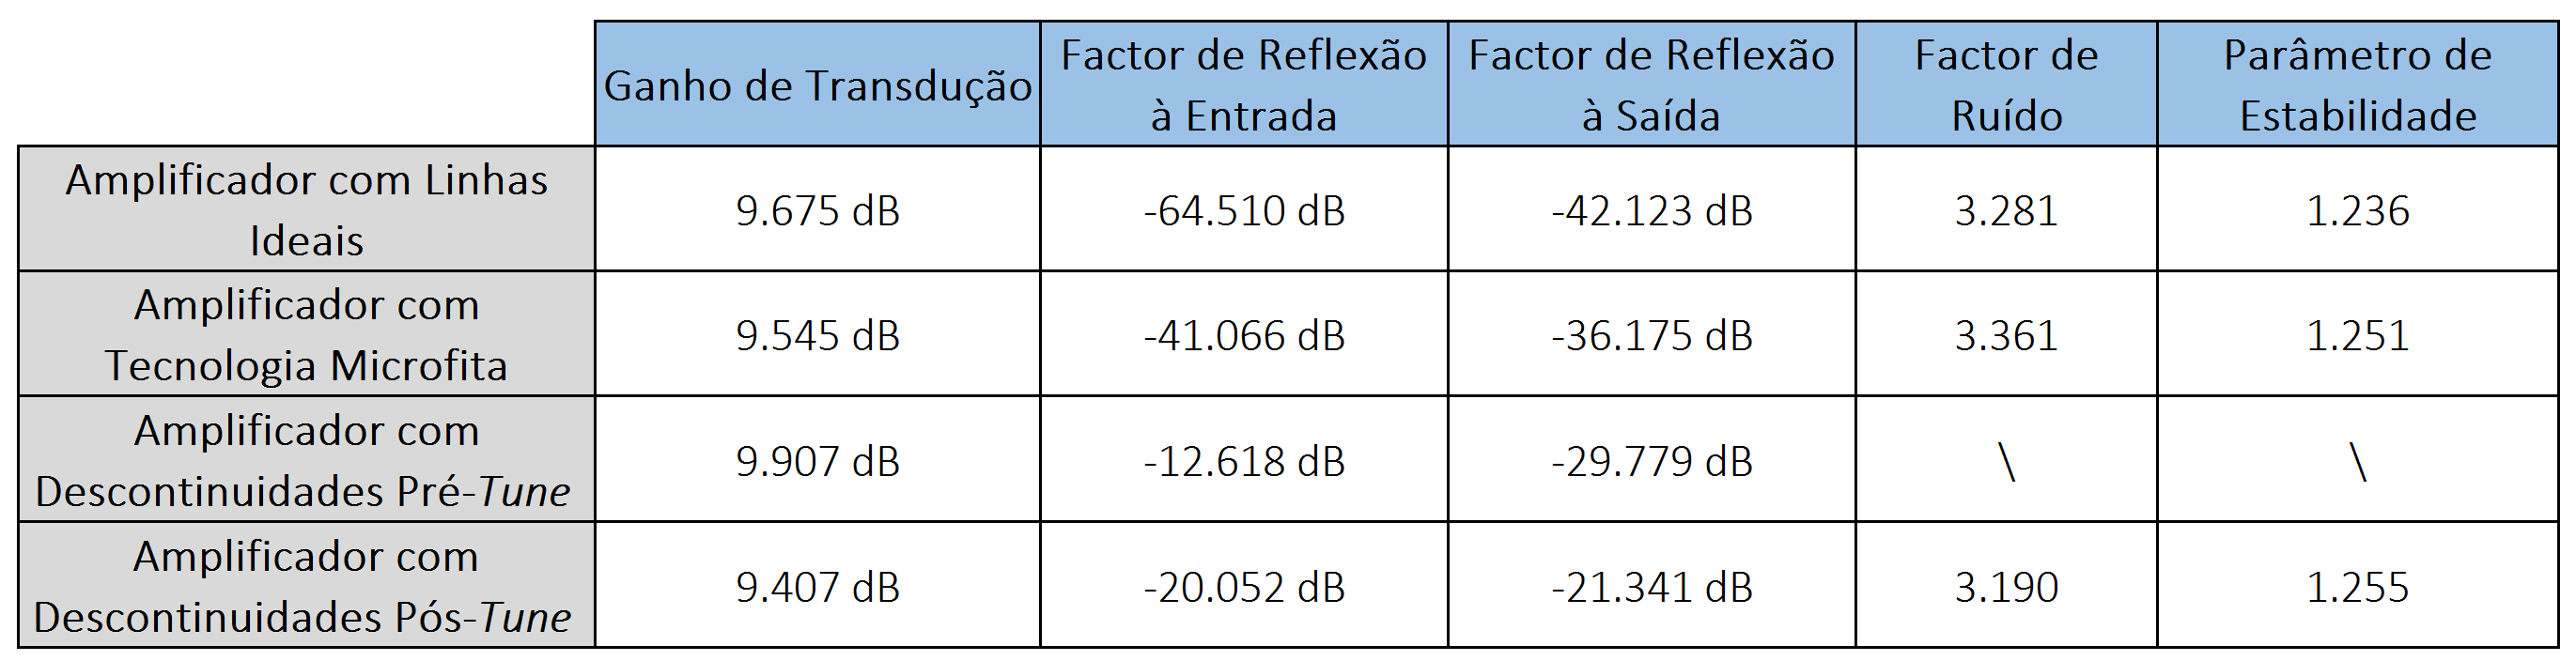
\includegraphics[keepaspectratio=true, scale=0.45]{exps/compfinal}
	\label{tab:comparacao_final}
\end{table}

Um dos objectivos do projecto do amplificador, tal como se pode ver na Tabela \ref{tab:car}, era obter um ganho de transdução máximo, tendo sido realizada a adaptação conjugada simultânea com esse objectivo, sendo que o valor esperado para o ganho de transdução seria o apresentado na Tabela \ref{tab:param_S} como MAG. Como se pode observar, o valor obtido é bastante próximo e apresenta uma diferença de $0.257$ dB, que é causada pelas perdas nas microfitas. Não existia qualquer tipo de especificação em relação ao factor de ruído, no entanto, em relação ao amplificador com linhas ideais, o projecto final do amplificador (amplificador sem descontinuidades pós-\textit{tune}) apresenta um valor mais satisfatório, diminuindo ainda mais a importância da diferença entre o ganho de transdução dos dois amplificadores (linhas ideais e projecto final).

Os valores de ambos os factores de reflexão são muito inferiores em módulo em relação aos simulados no amplificador com linhas ideais. Isto acontece pois o objectivo durante a utilização da ferramenta de optimização (\texttt{TUNE}) era maximizar o valor do ganho de transdução, manter o máximo do ganho de transdução e os mínimos de ambos os factores de reflexão centrados na frequência 22 GHz, sem comprometer em demasia os valores mínimos de ambos os factores de reflexão. É preciso ter em conta que, por exemplo, obter um factor de reflexão à entrada com o valor de -79 dB e à saída com um valor de -10 dB é muito menos favorável que ter ambos os factores de reflexão a -15 dB. Assim, foi definido como valor mínimo aceitável para ambos os factores de reflexão -15 dB, no entanto, enquanto o processo de optimização avançava, a precisão do \texttt{TUNE} era aumentada progressivamente. Foram então obtidos os valores apresentados na Tabela \ref{tab:comparacao_final}.

\subsubsection{b) Substituição do transístor e condensadores}

Em primeiro lugar, tem de se determinar as dimensões dos condensadores e, sabendo que estes têm um valor de 39 pF, foi necessário recorrer a uma \textit{datasheet} de condensadores com esse valor, sendo escolhida a do elemento \texttt{KEMET Part Number: C0402C390J5GACTU}. As suas dimensões podem ser consultadas na Figura \ref{fig:capacitor}, e são calculados na Equação \ref{eq:capacitor2}.

\begin{figure}[H]
	\centering
	\includegraphics[keepaspectratio=true, scale=0.45]{teoricas/capacitor}
	\vspace{-0.5em}
	\caption{Dimensões dos condensadores.}
	\vspace{-9mm}
	\label{fig:capacitor}
\end{figure}

\vspace{-3mm}
\begin{equation}
	W_{\texttt{MGAP}} = W_{\textit{datasheet}} + \lvert\text{tolerance}\rvert = 0.505~\text{mm} ~~ \text{e} ~~ S_{\texttt{MGAP}} = L_{\textit{datasheet}} + \lvert\text{tolerance}\rvert = 1.06~\text{mm}.
	\label{eq:capacitor2}
\end{equation}

\vspace{-1mm}
Pode-se então determinar a dimensão dos elementos \texttt{MGAP} a utilizar para substituir os condensadores. No entanto, como os condensadores têm uma largura diferente da do canal onde estão a ser inseridos, é necessário usar \texttt{MSTEP's} para adaptar os condensadores ao canal.

Para substituir o transístor pelo elemento \texttt{MGAP} tem de se calcular as dimensões de largura e comprimento a utilizar. Ao se consultar o \textit{datasheet} do transístor é possível concluir que o encapsulamento tem $1.76$ mm, pelo que é necessário uma dimensão S do elemento \texttt{MGAP} ligeiramente superior, diga-se $2.5$ mm. Em relação à largura do \texttt{MGAP}, esta tem de coincidir com o tamanho dos \textit{pins} da \textit{gate} e do \textit{dreno} do transístor, $0.51$ mm. Mais uma vez, como a dimensão da largura do \texttt{MGAP} não é igual à do canal em que este será inserido, foram usados elementos\texttt{MSTEP} para adaptar o canal.

O circuito que resulta destas substituições dos condensadores e transístores pode ser observado na Figura \ref{fig:Circuito_layout}.

\begin{figure}[H]
	\centering
	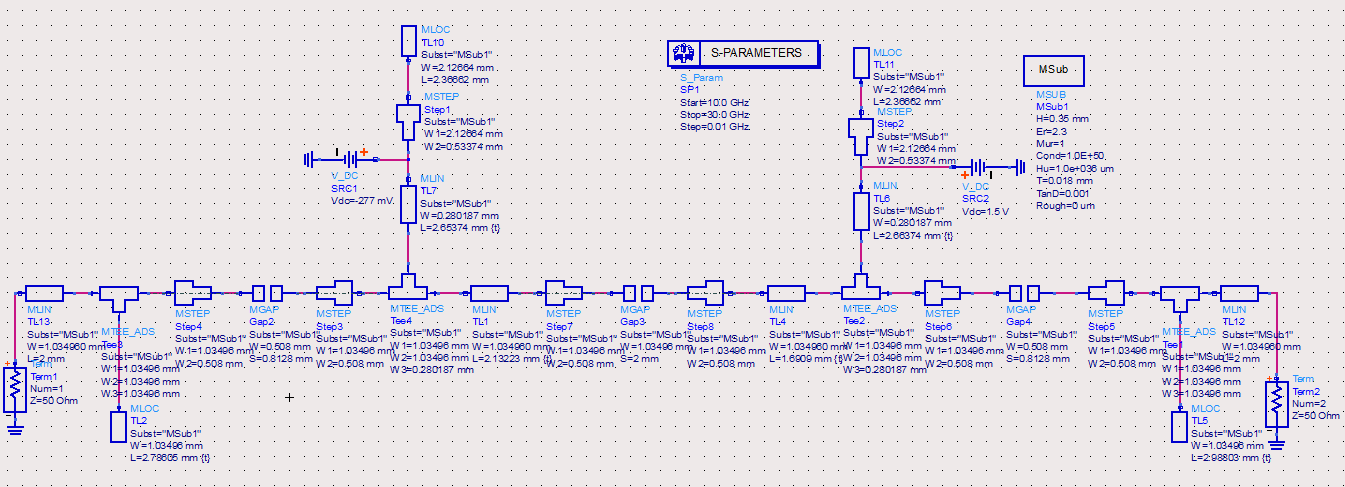
\includegraphics[keepaspectratio=true, scale=0.45]{exps/Circuito_layout}
	\vspace{-0.5em}
	\caption{Circuito que corresponde ao projecto de \textit{layout} do amplificador.}
	\vspace{-0.8em}
	\label{fig:Circuito_layout}
\end{figure}

Ao ter o circuito totalmente projectado, é possível usar a ferramenta \texttt{layout} do ADS para construir o \textit{layout} do circuito, que pode ser observado na Figura \ref{fig:layout}.

\begin{figure}[H]
	\centering
	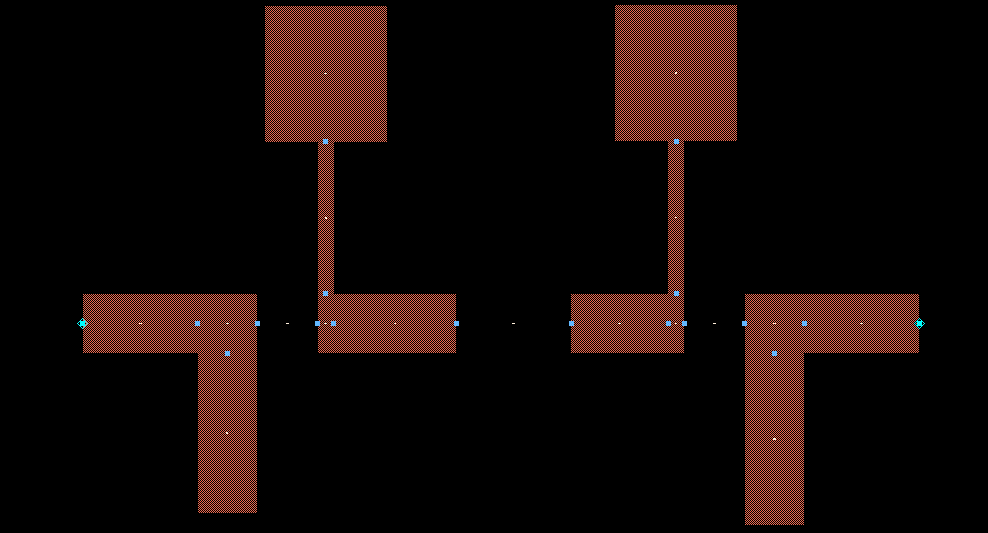
\includegraphics[keepaspectratio=true, scale=0.45]{exps/layout}
	\vspace{-0.5em}
	\caption{\textit{Layout} do amplificador.}
	\vspace{-0.8em}
	\label{fig:layout}
\end{figure}

\section{Conclusões}

\end{document}